\begin{frame}{Alert Production}

\only<1-3>{
  \textbf{LDM-503-1: Alert generation milestone}

  \begin{itemize}

    \item{First (equal) post-replan, NSF-visible milestone hit by the
    project.}
    \item{Demonstrating a \textit{end-to-end} alert production pipeline.}
    \item{Milestone succesful (\citeds{DMTR-53})!}
    \invisible<1>{

      \item{Effort to upgrade, enhance, expand, etc the AP pipeline
      will continue throughout construction.}
      \item{Currently focusing on improved source association routines, and
      making it a more idiomatically ``stack-like'' system.}
      \item{Will form the basis of QA efforts going forward.}

    }
  \end{itemize}
}

\invisible<1-2>{
\textbf{SkyWcs}

  \begin{itemize}
    \item{Entirely new back-end for WCS (pixel to/from sky coordinate)
    transformations.}
    \item{\textit{Months} of effort, just merged a couple of weeks ago.}
  \end{itemize}

}
\end{frame}


\begin{frame}{Alert Production}

\only<1-2>{
  \textbf{Moving Objects}

  \begin{itemize}

    \item{Awesome new MOPS linking algorithm under development.} \item{In the
    process of reconsidering our moving objects strategy and integrating more
    closely with the Minor Planet Center. Watch for more soon...}

  \end{itemize}
}

\invisible<1>{
  \textbf{Jointcal}

  \vspace{-0.5cm}
  \begin{columns}
    \begin{column}{0.72\textwidth}
      \begin{itemize}
        \item{Simultaneous astro- and photometric fitting to source lists derived
        from multiple images.}
        \item{The all new, much improved, more generic replacement for the
        HSC-specific meas\_mosaic.}
        \item{Still getting the rough edges smoothed off... aiming to have this
        entirely supersede meas\_mosaic (which will be removed from the stack
        entirely) really soon now.}
      \end{itemize}
    \end{column}

    \begin{column}{0.28\textwidth}
      \begin{center}
        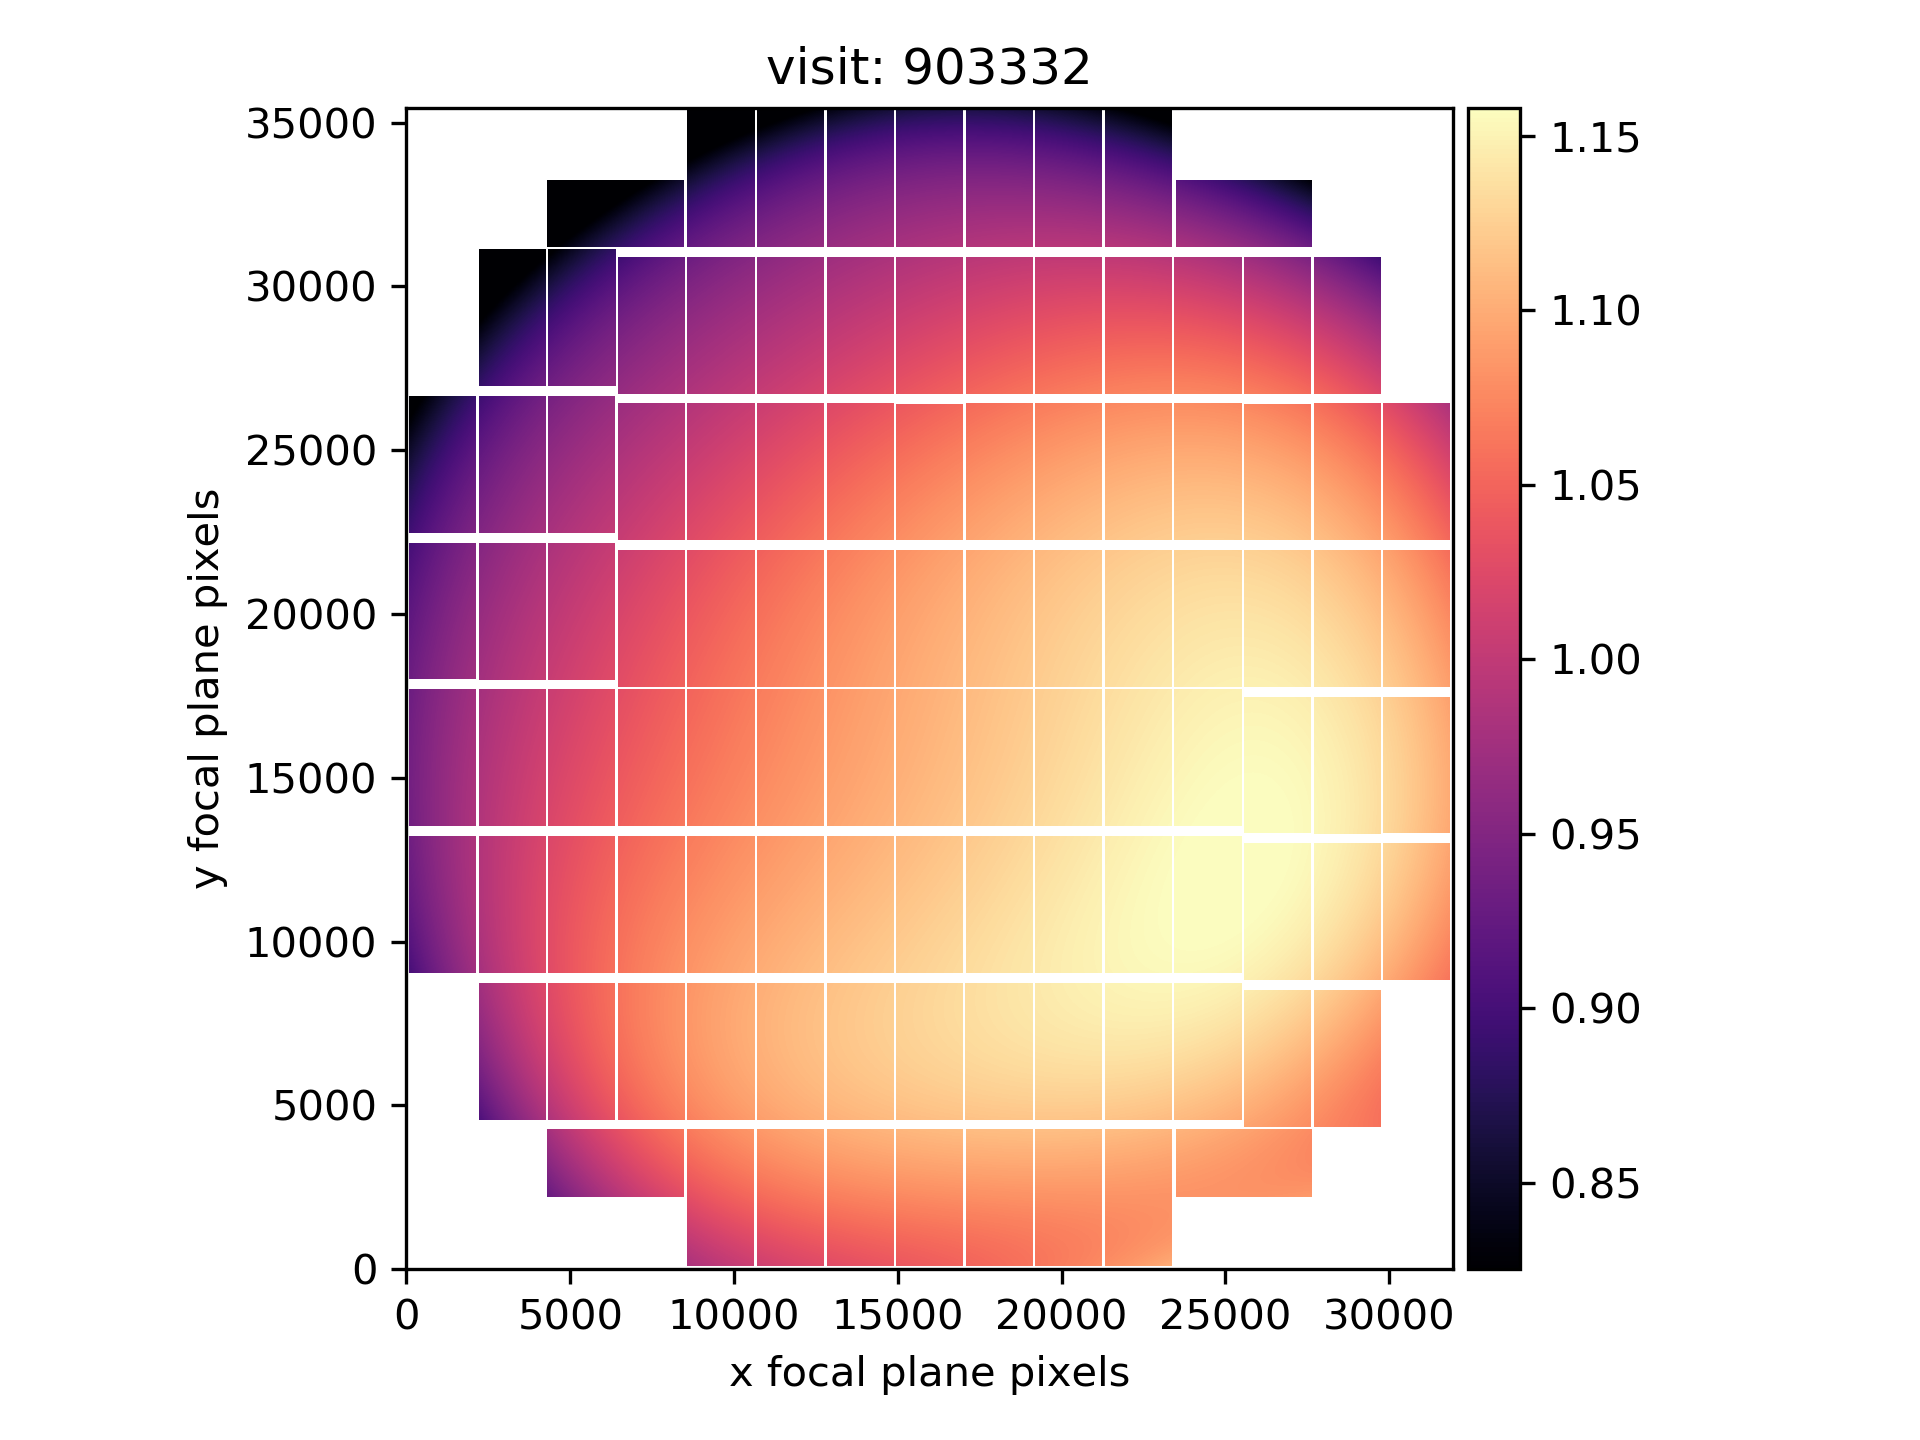
\includegraphics[width=1.0\textwidth]{figures/jointcal.png}\\
        \tiny Figure: Parejko.
      \end{center}
    \end{column}
  \end{columns}
}

\end{frame}

\begin{frame}{Alert Production}

\only<1-2>{
  \textbf{Alert Distribution}
  \begin{columns}

    \begin{column}{0.75\textwidth}
      \vspace{-0.5cm}
      \begin{itemize}

        \item{Prototype alert distribution system using Kafka \& AVRO; benchmark
        results on \citeds{DMTN-028}.}

        \item{Moving on to start prototyping filtering technologies and the
        ``mini-broker''.}
      \end{itemize}
    \end{column}

    \begin{column}{0.25\textwidth}
      \vspace{-0.5cm}
      \begin{center}
        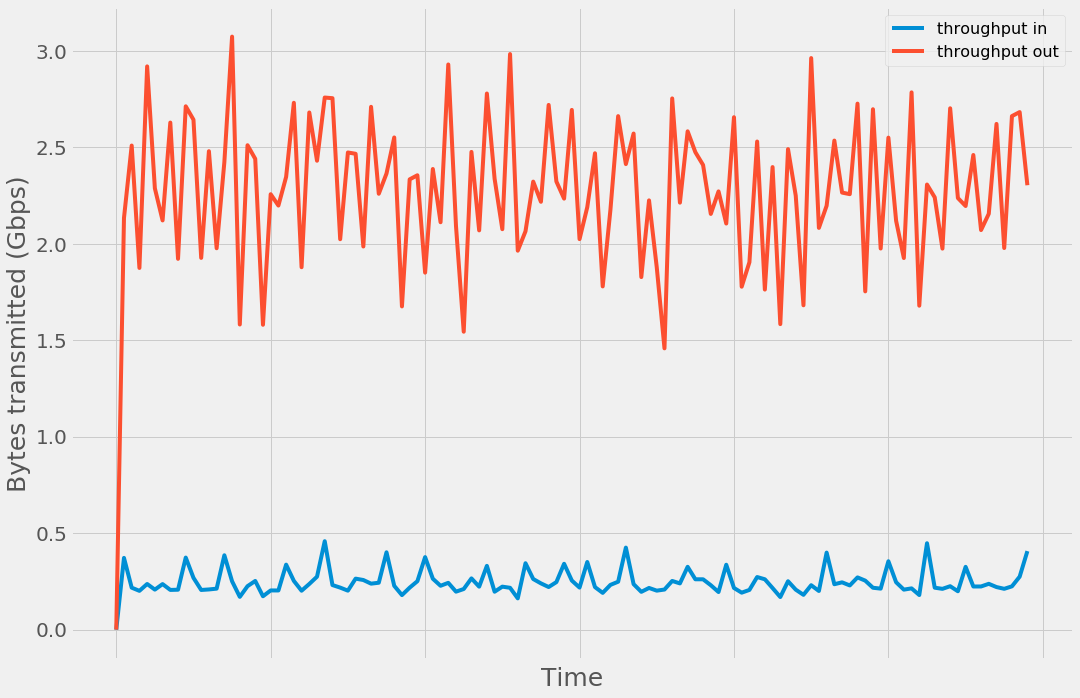
\includegraphics[width=1.0\textwidth]{figures/kafka.png}\\
        \tiny Figure: Patterson.
      \end{center}
    \end{column}

  \end{columns}
}

\invisible<1>{
  \vspace{-0.5cm}
  \textbf{DCR-matched Template Generation}
  \begin{columns}

    \begin{column}{0.25\textwidth}
      \vspace{-0.5cm}
      \begin{center}
        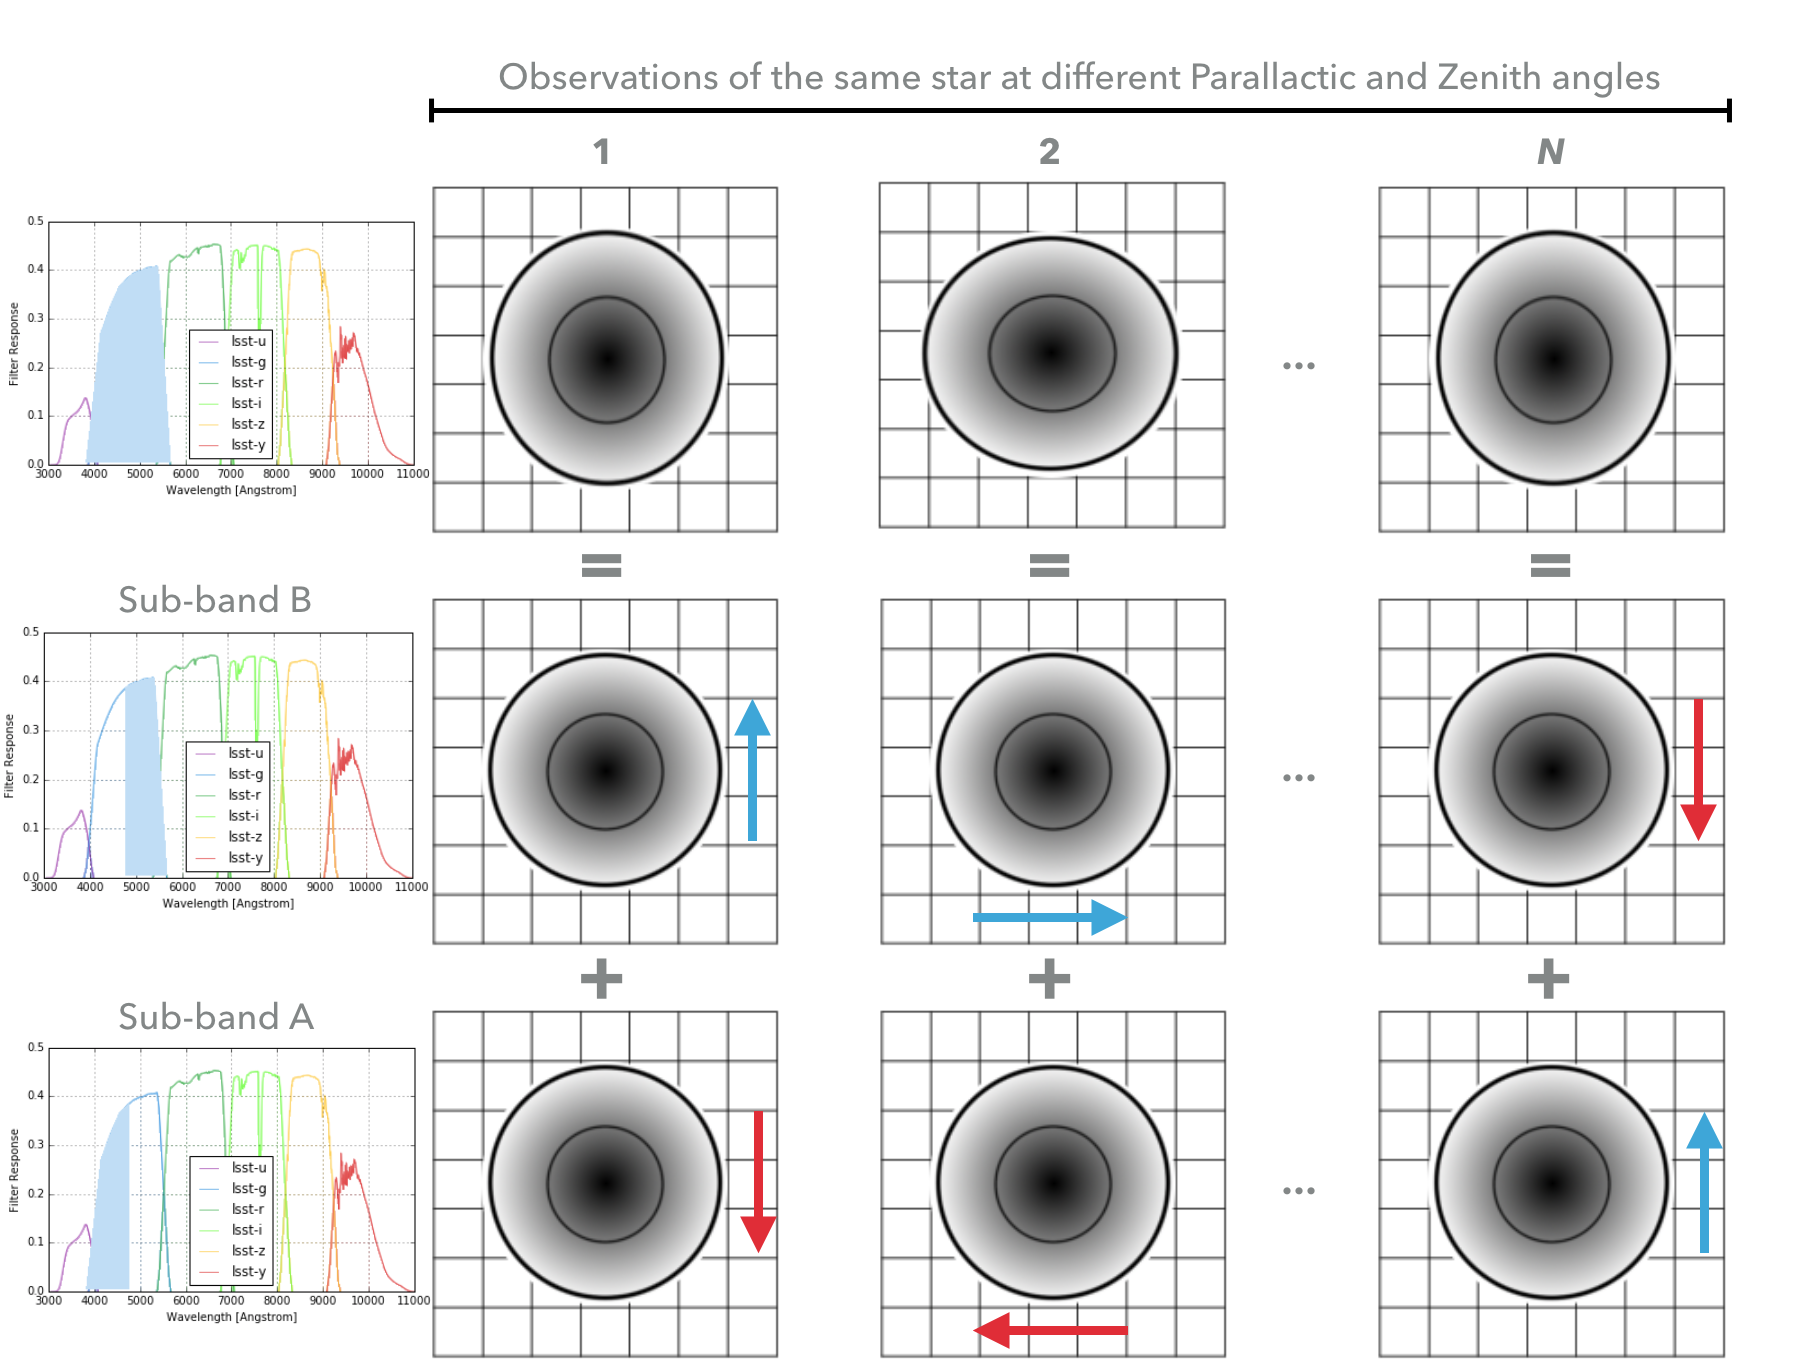
\includegraphics[width=1.0\textwidth]{figures/dcr.png}\\
        \tiny Figure: Sullivan.
      \end{center}
    \end{column}

    \begin{column}{0.75\textwidth}
      \begin{itemize}
        \item{Initial algorithm for making differential chromatic
        refraction-matched templates about to be come available in the stack.}
        \item{Moving on to address variable PSFs, journal publication, and
        large-scale, real-world testing.}
      \end{itemize}
    \end{column}
  \end{columns}
}
\end{frame}

\begin{frame}{Data Release Production}

\only<1-2>{
  \textbf{LDM-503-2: HSC reprocessing milestone}

  \begin{itemize}

    \item{First (equal) post-replan, NSF-visible milestone hit by the project.}
    \item{Joint effort to reprocess (LDF team) and analyze (DRP team) HSC data
    under operations-like conditions}
    \item{Milestone successful \citeds{DMTR-51}!}

  \end{itemize}
}

\invisible<1>{
  \textbf{``Warp Compare'' coadds}

  \begin{itemize}
    \item{New algorithm to robustly reject artefacts when coadding images.}
    \item{Now default for HSC processing; stack-wide default to be RFCed soon.}
  \end{itemize}

  \begin{center}
  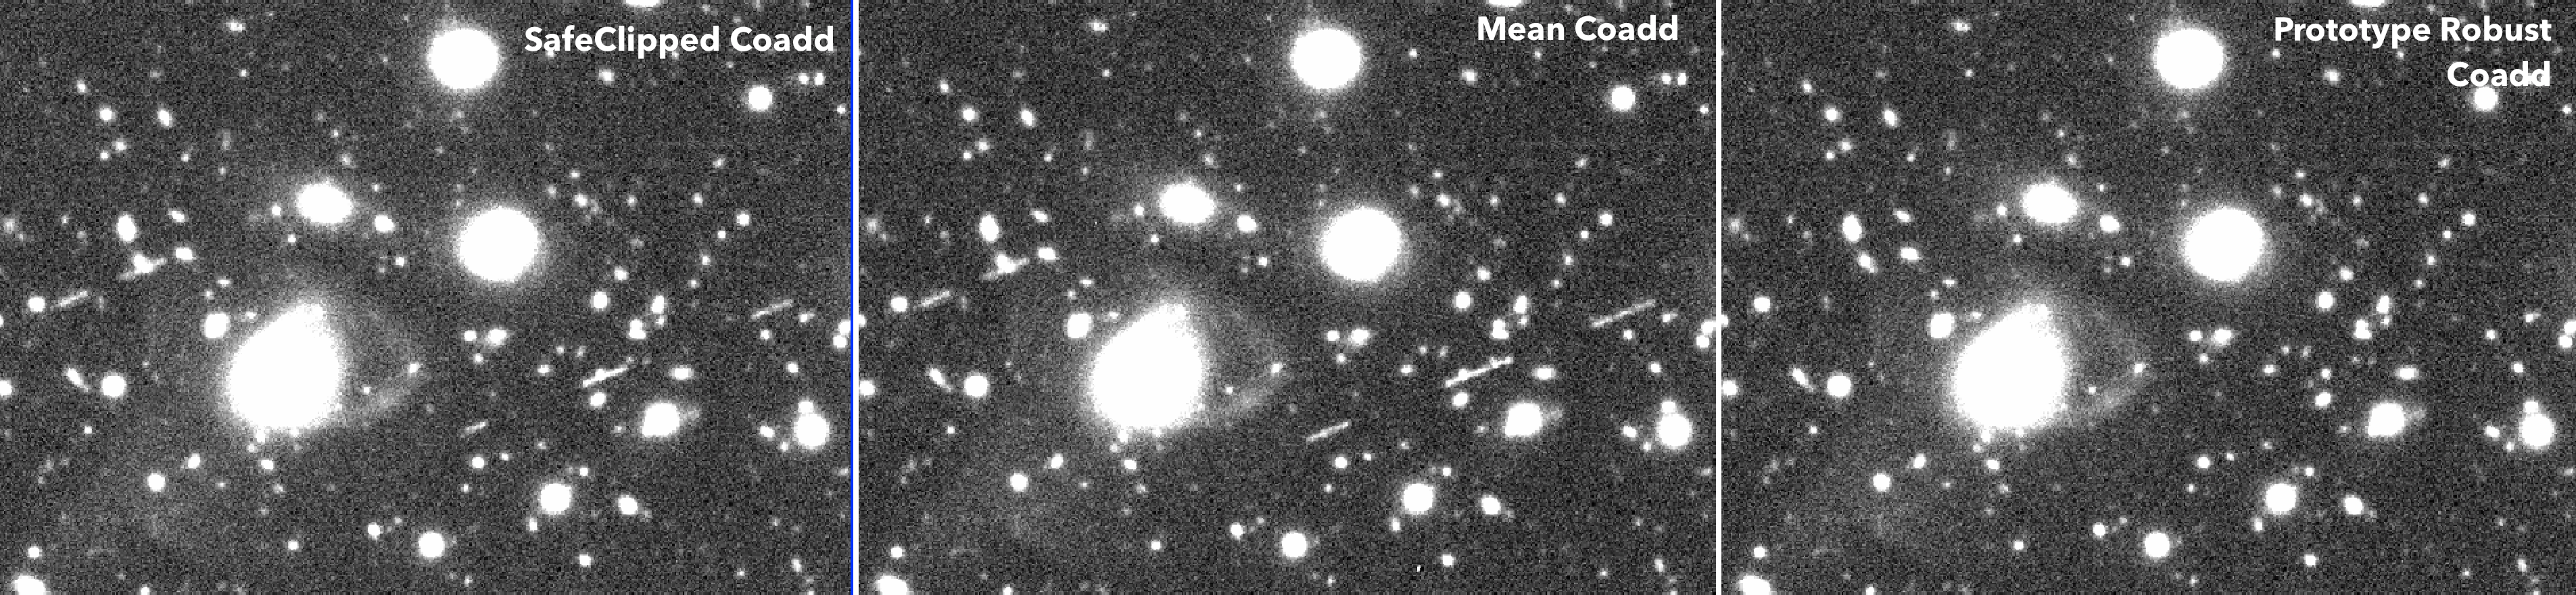
\includegraphics[width=0.5\textwidth]{figures/warpcompare.png}\\
  \tiny Figure: AlSayyad.
  \end{center}
}

\end{frame}

\begin{frame}{Data Release Production}

\textbf{Scarlet: the ``new deblender''}

\begin{itemize}
 \only<1-2>{\item{Key pipeline component; separates overlapping astrophysical objects
 into their constitutent components for measurement.}
  \item{Recent activities:
    \begin{itemize}
      \item{Prototype code developed over the last $\sim$year with exceptionally
      promising results.}
      \item{Journal paper describing the algorithm submitted.}
    \end{itemize}
  }}
  \invisible<1>{\item{Coming up:
    \begin{itemize}
      \item{Performance optimization.}
      \item{Demonstrate performance at-scale on real data with real
      pathologies.}
      \item{Considering how deblender results should affect our approach to
      measurement.}
    \end{itemize}
  }}
\end{itemize}

\begin{center}
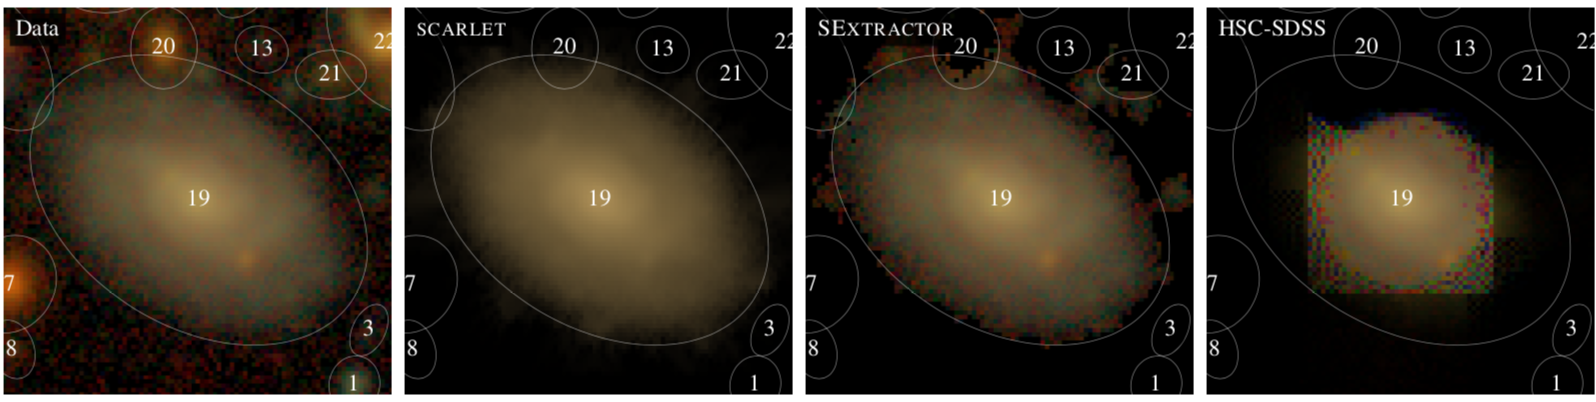
\includegraphics[width=0.5\textwidth]{figures/scarlet.png}\\
\tiny Figure: Melchior et al., 2018
\end{center}

\end{frame}

\begin{frame}{Data Release Production}

\only<1-2>{
  \textbf{``Clever'' coadds}
  \begin{itemize}
    \item{Investigating to what extent we could refine our coaddition techniques
    to enable us to meet our requirements on galaxy shear by measuring
    \textit{only} on coadds (i.e., avoiding the cost \& complexity of MultiFit).}
    \item{Still a work in progress... watch this space.}
  \end{itemize}
}

\invisible<1>{
\textbf{Calibration products \& Auxiliary Telescope}
  \begin{itemize}
    \item{First version of calibration products pipeline added to stack: the
    cp\_pipe package.}
    \item{Currently working on Brighter-Fatter mitigation.}
    \item{Expecting to start on collimated beam projector analysis in F17.}
    \item{Major push on AuxTel spectrophotometric pipeline this year:
    intensive planning in January; tests planned for May \& August; aiming for
    prototype pipeline late summer followed by stack integration.}
  \end{itemize}
}

\end{frame}

\begin{frame}{Data Release Production}

\only<1-2>{
\textbf{``QA'' on HSC data}
\begin{itemize}

  \item{Continued effort to flush out and eliminate all the weird issues that
  crop up when we run the DRP pipelines at scale.}
  \item{Plus: new tooling! Come and learn all about it at the Wednesday
  morning session.}
\end{itemize}
}

\invisible<1>{
\textbf{Do(ough)nuts!}
  \begin{itemize}
    \item{...or rather: using out-of-focus images of stars to measure the
    wavefront, then using that to derive the PSF due to the optical system (as
    opposed to the atmosphere).}
    \item{See results in \citeds{DMTN-064}.}
  \end{itemize}

  \vspace{-0.2cm}
  \begin{center}
  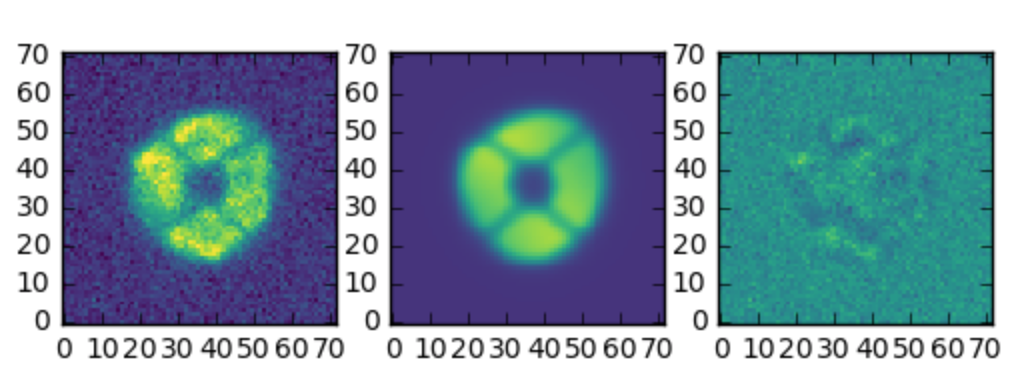
\includegraphics[width=0.5\textwidth]{figures/donut.png}\\
  \tiny Figure: Meyers, \citeds{DMTN-064}
  \end{center}
}

\end{frame}

\begin{frame}{Data Release Production}

\textbf{And more!}
\begin{itemize}

  \item{Work getting started on:

    \begin{itemize}

      \item{Star-galaxy separation}
      \item{New galaxy fitting algorithm}

    \end{itemize}

    ... watch for news at the LSST 2018 Joint Technical Meeting.}

    \item{Lots of effort going into Butler Generation 3.}

\end{itemize}

\end{frame}
